% !TEX encoding = UTF-8 Unicode

\section{Friday}\index{Friday_lecture}
Before we give a proof of Schroder-Berstein theorem, we'd better review the definitions for one-to-one mapping and onto mapping. 
\begin{definition}[One-to-One/Onto Mapping]
If $f:A\mapsto B$, then 
\begin{itemize}
\item
$f$ is said to be \emph{onto} mapping if
\[
\forall b\in B,\exists a\in A\mbox{ s.t. }f(a)=b;
\]
\item
$f$ is said to be \emph{one-to-one} mapping if
\[
\forall a,b,\in A, f(a)=f(b)\implies a=b.
\]
\end{itemize}
\end{definition}
The Fig.(\ref{Fig:1:1}) shows the examples of one-to-one/onto mappings.
\begin{figure}
\centering  
\subfigure[A one-to-one but not onto mapping]{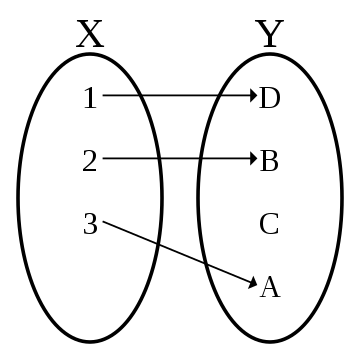
\includegraphics[width=0.45\linewidth]{week1/f_1}}
\subfigure[A one-to-one onto mapping]{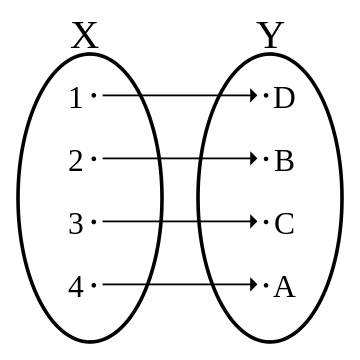
\includegraphics[width=0.45\linewidth]{week1/f_2}}
\subfigure[A onto but not one-to-one mapping]{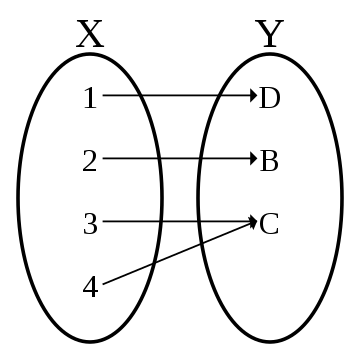
\includegraphics[width=0.45\linewidth]{week1/f_3}}
\subfigure[Neither a one-to-one nor onto mapping]{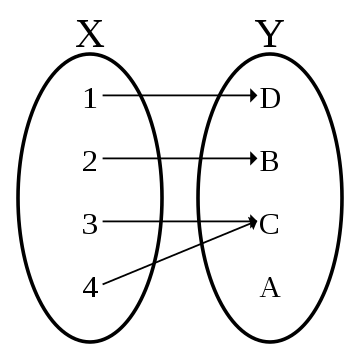
\includegraphics[width=0.45\linewidth]{week1/f_4}}
\caption{Illustrations of one-to-one/onto mappings}\label{Fig:1:1}
\end{figure}
\subsection{Proof of Schroder-Berstein Theorem}
Before the proof, note that in this lecture we abuse the notation $fg$ to denote the composite function $f\circ g$, but in the future $fg$ will refer to other meanings.
\paragraph{Intuition from Fig.(\ref{Fig:1:2})}
The proof for this theorem is constructive. Firstly Fig.(\ref{Fig:1:2}) gives us the intuition of the proof for this theorem. 
\begin{figure}
\centering
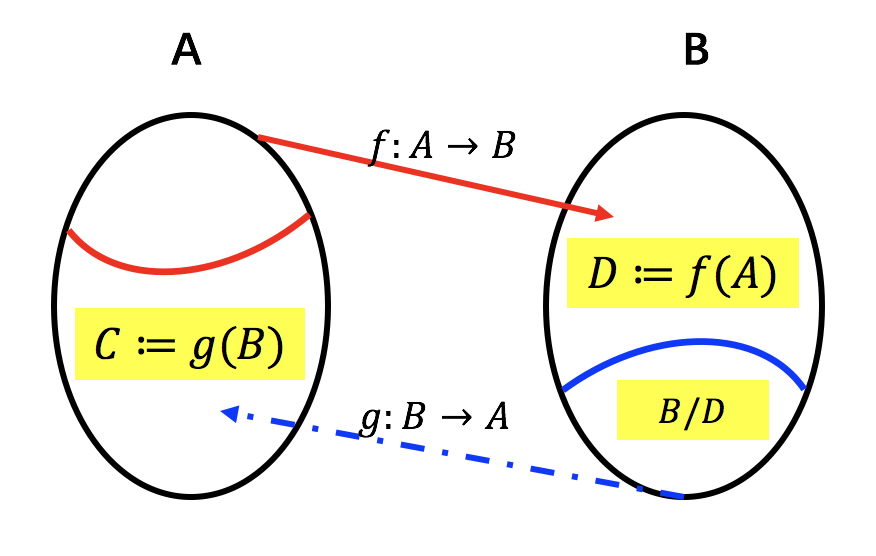
\includegraphics[width=0.65\linewidth]{week1/f_5}
\caption{Illustration of Schroder-Berstein Theorem}
\label{Fig:1:2}
\end{figure}
Let $f: A\mapsto B$ and $g: B\mapsto A$ be two one-to-one mappings, and $D,C$ are the image from $A,B$ respectively. Note that
\begin{quotation}
if the set $B\setminus D$ is empty, then $D=B=f(A)$ with $f$ being the one-to-one mapping, which implies $f$ is one-to-one onto mapping. In this case the proof is complete.
\end{quotation}
Hence it suffices to consider the case $B\setminus D$ is non-empty. Thus $B\setminus D$ is the ``\emph{trouble-maker}''. To construct a one-to-one onto mapping from $A$, we should study the subset $g(B\setminus D)$ of $A$ (which can also be viewed as a \textit{trouble-maker}). Moreove, we should study the subset $gf[g(B\setminus D)]$ (which is also a \textit{trouble-maker})... so on and so forth. Therefore, we should study the \textit{union of these trouble makers}, i.e., we define
\[
\begin{array}{llll}
A_1:=g(B\setminus D),
&
A_2:=gf(A_1),
&
\cdots,
&
A_{n}:=gf(A_{n-1}),
\end{array}
\]
Then we study the union of infinite sets
\[
S:=A_1\bigcup A_2\bigcup\cdots\bigcup A_n\bigcup\cdots
\]
Define
\[
F(a)=\left\{
\begin{aligned}
f(a),&\quad a\in A\setminus S\\
g^{-1}(a),&\quad a\in S
\end{aligned}
\right.
\]
We claim that $F:A\mapsto B$ is one-to-one onto mapping.
\paragraph{$F$ is onto mapping} Given any element $b\in B$, it follows two cases:
\begin{enumerate}
\item
$g(b)\in S$. It implies $F(g(b))=g^{-1}(g(b))=b$.
\item
$g(b)\notin S$. It implies $b\in D$, since otherwise $b\in B\setminus D\implies g(b)\in g(B\setminus D)\subseteq S$, which is a contradiction. $b\in D$ implies that $\exists a\in A$ s.t. $f(a)=b$. 

Then we study the relationship between $gf(S)$ and $S$. Verify by yourself that
\[
S=g(B\setminus D)\bigcup gf(S)
\]
With this relationship, we claim $a\notin S$, since otherwise $a\in S\implies gf(a)\in S$, but $gf(a)=g(b)\notin S$, which is a contradiction.

Hence, $F(a)=f(a)=b$.
\end{enumerate}
Hence, for any element $b\in B$, we can find a element from $A$ such that the mapping for which is equal to $b$, i.e., $F$ is onto mapping.
\paragraph{$F$ is one-to-one mapping}
Assume not, verify by yourself that the only possibility is that $\exists a_1\in A\setminus S$ and $a_2\in S$ such that $F(a_1)=F(a_2)$, i.e., $f(a_1)=g^{-1}(a_2)$, which follows 
\begin{equation}
gf(a_1)=a_2\in S=A_1\bigcup A_2\bigcup\cdots\label{Eq:1:1}
\end{equation}
We claim that Eq.(\ref{Eq:1:1}) is false. Note that 
$gf(a_1)\notin A_1:=g(B\setminus D)$, since otherwise $f(a_1)\in B\setminus D$, which is a contradiction; note that $gf(a_1)\notin A_2$, since otherwise $gf(a_1)\in  gfg(B\setminus D)\implies a_1\in g(B\setminus D)=A_1\subseteq S$, which is a contradiction.

Applying the similar trick, we wil show that $gf(a_1)\notin A_k$ for $k\ge 1$. Hence, Eq.(\ref{Eq:1:1}) is false, the proof is complete.
\begin{example}
Given two sets $A:=(0,1]$ and $B:=[0,1)$. Now we apply the idea in the proof above to construct a one-to-one onto mapping from $A$ to $B$:
\begin{itemize}
\item
Firstly we construct two one-to-one mappings:
\[
\begin{aligned}
f:&A\mapsto B\\
f(x)&=\frac{1}{2}x
\end{aligned}
\qquad
\begin{aligned}
g:&B\mapsto A\\
g(x)&=x
\end{aligned}
\]
\item
It follows that $B\setminus D=(\frac{1}{2},1)$, $gf(B\setminus D)=(\frac{1}{4},1)$, so on and so forth.
\[
S=(\frac{1}{2},1)\bigcup (\frac{1}{4},1)\bigcup\cdots
\]
\item
Hence, the one-to-one onto mapping we construct is
\[
F(x)=\left\{
\begin{aligned}
\frac{1}{2}x,&\quad x\in A\setminus S\\
x,&\quad x\in S
\end{aligned}
\right.
\]
\item
Conversely, to construct the inverse mapping, we define
\[
\begin{array}{ll}
f(x)=x
&
g(x)=\frac{1}{2}x
\end{array}
\]
\item
It follows that $D=(0,1)$, $B\setminus D=\{1\}$. Then
\[
S=\left\{\frac{1}{2}\right\}\bigcup\cdots=\left\{\frac{1}{2},\frac{1}{4},\cdots\right\}
\]
\item
Hence, the function we construct for inverse mapping is
\[
F(x)=\left\{
\begin{aligned}
x,&\quad x\ne\frac{1}{2^m}\\
2x,&\quad x=\frac{1}{2^m}
\end{aligned}
\right.
\qquad
(m=1,2,3,\dots)
\]
\end{itemize}
\end{example}
\subsection{Connectedness of Real Numbers}
There are two approaches to construct real numbers. Let's take $\sqrt{2}$ as an example.
\begin{enumerate}
\item
The first way is to use \emph{Dedekind Cut}, i.e., every non-empty subset has a least upper bound. Therefore, $\sqrt{2}$ is actually the least upper bound of a non-empty subset
\[
\{x\in\mathbb{Q}\mid x^2<2\}.
\]
\item
Another way is to use \emph{Cauchy Sequence}, i.e., every Cauchy sequence is convergent. Therefore, $\sqrt{2}$ is actually the limit of the given sequence of decimal approximations below:
\[
\{1,1.4,1.41,1.414,1.4142,\dots\}
\]
\end{enumerate}
We will use the second approach to define real numbers. Every real number $r$ essentially represents a collection of cauchy sequences with limit $r$, i.e.,
\[
r\in\mathbb{R}
\implies
\left\{
\{x_n\}_{n=1}^\infty\middle|
\lim_{n\to\infty}x_n=r
\right\}
\]
Let's give a formal definition for cauchy sequence and a formal definition for real number.
\begin{definition}[Cauchy Sequence]
\begin{itemize}
\item
Any sequence of rational numbers $\{x_1,x_2,\cdots\}$ is said to be a \emph{cauchy sequence} if for every $\epsilon>0$, $\exists N$ s.t. $|x_n-x_m|<\epsilon$, $\forall m,n\ge N$
\item
Two cauchy sequences $\{x_1,x_2,\dots\}$ and $\{y_1,y_2,\dots\}$ are said to be \emph{equivalent} if for every $\epsilon>0$, there $\exists N$ s.t. $|x_n-y_n|<\epsilon$ for $\forall n\ge N$.
\item
A real number is a \emph{collection} of \emph{equivalent} cauchy sequences. It can be represented by a cauchy sequence:
\[
x\in\mathbb{R}\sim\{x_1,x_2,\dots,x_n,\dots\},
\]
where $x_j$ is a rational number.
\end{itemize}
\end{definition}
\begin{remark}
Let $\xi_{\mathbb{Q}}$ denote a collection of any cauchy sequences. Then once we have equivalence relation, the whole collection $\xi_{\mathbb{Q}}$ is partitioned into several disjoint subsets, i.e., equivalence classes. Hence, the real number space $\mathbb{R}$ are the equivalence classes of $\xi_{\mathbb{Q}}$.
\end{remark}

The real numbers are well-defined, i.e., given two real numbers $x\sim\{x_1,x_2,\dots\}$ $y\sim\{y_1,y_2,\dots\}$, we can define add and multiplication operator.
\begin{align*}
x+y&\sim\{x_1+y_1,x_2+y_2,\dots\}\\
x\cdot y&\sim\{x_1\cdot y_1,x_2\cdot y_2,\dots\}
\end{align*}
We will show how to define $x>0$ in next lecture, this construction essentially leads to the lemma below:
\begin{proposition}
$\mathbb{Q}$ are dense in $\mathbb{R}$.
\end{proposition}
In the next lecture we will also show the completeness of $\mathbb{R}$:
\begin{theorem}
$\mathbb{R}$ is complete, i.e., every cauchy sequence of real numbers converges.
\end{theorem}
Recommended Reading:
\begin{quotation}
Prof. Katrin Wehrheim, MIT Open Course, Fall 2010,
Analysis I Course Notes, Online avaiable: 
\begin{verbatim}
https://ocw.mit.edu/courses/mathematics
/18-100b-analysis-i-fall-2010/readings-notes/MIT18_100BF10_Const_of_R.pdf
\end{verbatim}
\end{quotation}















